\newpage
\section{Transport Layer}
\subsection{Overview of the transport layer}
Together with the network layer, the transport layer is the heart of the protocol hierarchy. The transport layer provides end-to-end connectivity across the network. 

\begin{figure}[!htb]
    \centering
    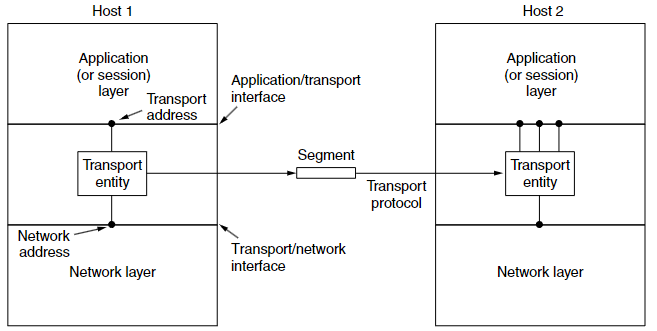
\includegraphics[width=0.42\textwidth]{pic/CN6/The network, transport, and application layers}
    \caption{The network, transport, and application layers}
\end{figure}

\subsubsection{The Transport Service}
Two types of transport service
\begin{itemize}
    \item Connection-oriented transport service
    \item Connectionless transport service
\end{itemize}
The transport code runs entirely on the users'machines, but the network layer mostly runs on the routers. The network service is generally unreliable. 

\subsubsection{Transit Units of Different Layers}
\begin{itemize}
    \item Transport layer: segment or TPDU (Transport Protocol Data Unit)
    \item Network layer: packet
    \item Data link layer: frame
    \item Physical layer: bit
\end{itemize}

\begin{figure}[!htb]
    \centering
    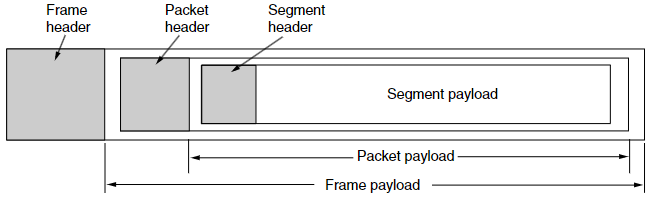
\includegraphics[width=0.42\textwidth]{pic/CN6/Nesting of segments, packets, and frames}
    \caption{Nesting of segments, packets, and frames}
\end{figure}

The Internet has two main protocols in the transport layer:
\begin{itemize}
    \item UDP (User Datagram Protocol, connectionless protocol): It does nothing beyond sending packets between applications. It typically runs in the operating system.
    \item TCP (connection-oriented protocol): It does almost everything. It makes connections and adds reliability with retransmission, along with flow control and congestion control.
\end{itemize}

\subsection{The internet transport protocols: UDP}
UDP: connectionless transport protocol. 

\begin{figure}[!htb]
    \centering
    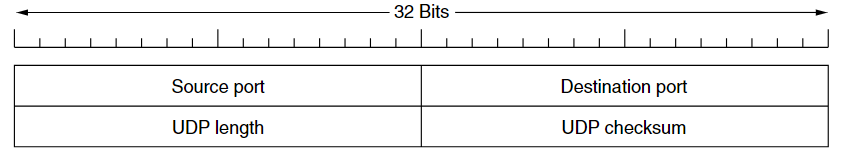
\includegraphics[width=0.42\textwidth]{pic/CN6/The UDP header}
    \caption{The UDP header}
\end{figure}

The two ports serve to identify the endpoints within the source and destination machines

\begin{itemize}
    \item UDP header (8 bytes)
    \begin{itemize}\small
        \item The UDP length field includes the 8-byte header and the data
        \subitem The minimum length is 8 bytes. The maximum length is 65,515 bytes. 
        \item The UDP checksum field (optional) is to provide extra reliability
        \subitem It checksums the header, data, and a conceptual IP pseudoheader
        \subitem The checksum algorithm is simply to add up all the 16-bit words (note here a word = 16 bits = 2 bytes) in one's complement and to take the one's complement of the sum.
    \end{itemize}
    \item The IPv4 pseudoheader
\end{itemize}
\begin{figure}[!htb]
    \centering
    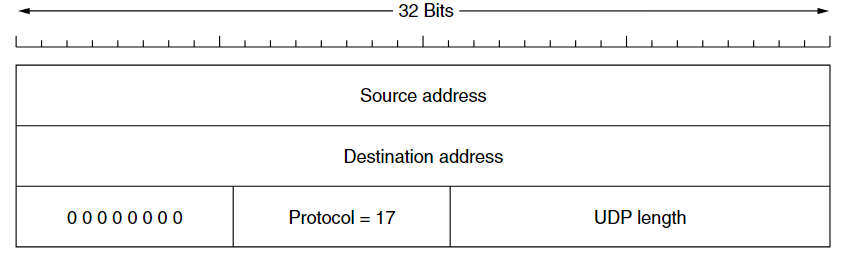
\includegraphics[width=0.42\textwidth]{pic/CN6/The IPv4 pseudoheader included in the UDP checksum.}
    \caption{The IPv4 pseudoheader included in the UDP checksum.}
\end{figure}

What UDP does not do: Flow control, congestion control, or retransmission upon receipt of a bad segment. 

What UDP does do:
\begin{itemize}
    \item To provide an interface to the IP protocol with the added feature of
    demultiplexing multiple processes using the ports.
    \item Optional end-to-end error detection (checksum)
\end{itemize}

The application uses the UDP protocol: 
\begin{itemize}
    \item DNS (Domain Name System, Chapter 7)
    \item SSDP (Simple Service Discovery Protocol)
\end{itemize}

\subsubsection{Real-Time Transport Protocol (RTP)}
It is a transport protocol but just happens to be implemented in the application layer.

Two aspects of real-time transport:
\begin{itemize}
    \item The RTP protocol for transporting audio and video data in packets
    \item How the receiver plays out the audio and video at the right time?
\end{itemize}

\begin{figure}[!htb]
    \centering
    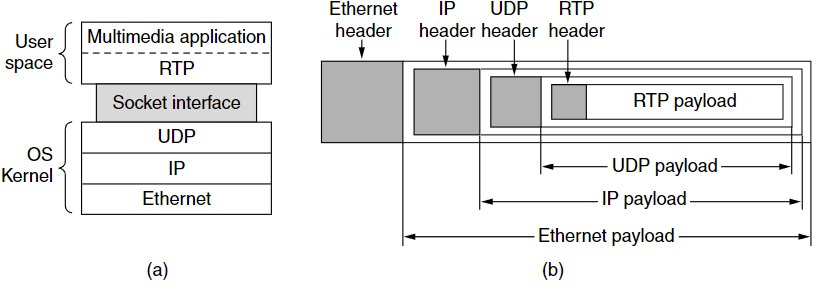
\includegraphics[width=0.42\textwidth]{pic/CN6/RTP.png}
    \caption{(a) The position of RTP in the protocol stack. (b) Packet nesting.}
\end{figure}

The basic function of RTP is to multiplex several real-time data streams onto a single stream of UDP packets

\begin{figure}[!htb]
    \centering
    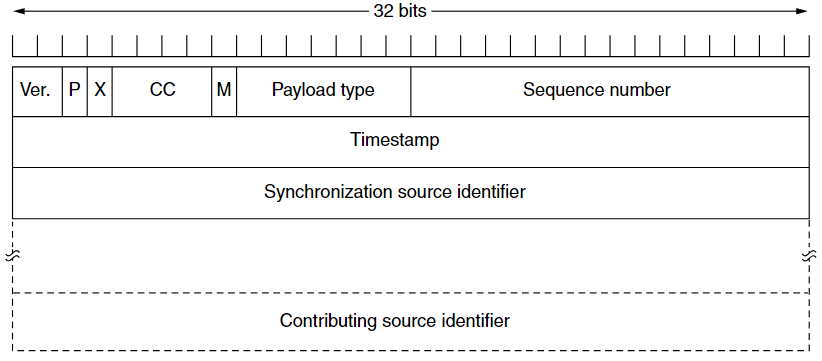
\includegraphics[width=0.42\textwidth]{pic/CN6/The RTP header}
    \caption{The RTP header}
\end{figure}
It consists of three 32- bit words and potentially some extensions
\begin{itemize}\small
    \item The Version field: 2
    \item The P bit indicates that the packet has been padded to a multiple of 4 bytes. The last padding byte tells how many bytes were added.
    \item The X bit indicates that an extension header is present.
    \item The CC field tells how many contributing sources are present, from 0 to 15.
    \item The M bit field is an application-specific marker bit.
    \item The Payload type field tells which encoding algorithm has been used.
    \item The Sequence number is just a counter that is incremented on each RTP packet sent. It is used to detect lost packets.
    \item The Timestamp is produced by the stream’s source to note when the 1st sample in the packet was made.
    \item The Synchronization source identifier tells which stream the packet belongs to.
    \item The Contributing source identifier, if any, are used when mixers are present in the studio.
\end{itemize}

\subsubsection{RTCP}
The RTCP (Real-time Transport Control Protocol) is a little sister protocol of RTP

Playout with Buffering and Jitter Control
\begin{figure}[!htb]
    \centering
    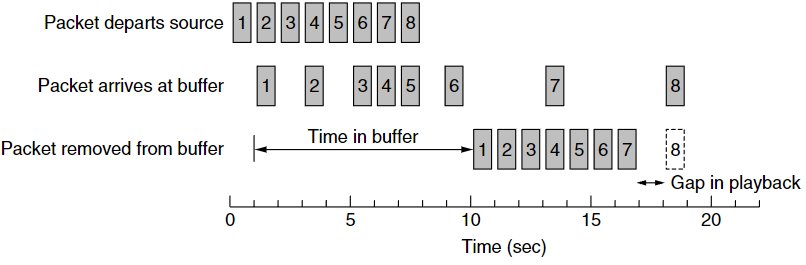
\includegraphics[width=0.42\textwidth]{pic/CN6/Smoothing the output stream by buffering packets}
    \caption{Smoothing the output stream by buffering packets}
\end{figure}

\subsection{The internet transport protocols: TCP}
TCP (Transmission Control Protocol) was designed to provide a reliable end-to-end byte stream over an unreliable internetwork. 

An internetwork may have wildly different topologies, bandwidths, delays, packet sizes, and other parameters in different parts.

\subsubsection{The TCP Service Model}
TCP service is obtained by both the sender and the receiver creating end points, called sockets. Each socket has a socket number (address) consisting of the IP addressing of the host and a 16-bit number local to that host, called a port.

All TCP connections are full duplex and point-to-point. TCP does not support multicasting and broadcasting. 

A TCP connection is a byte stream, not a message stream. (报文粘连问题)
\begin{figure}[!htb]
    \centering
    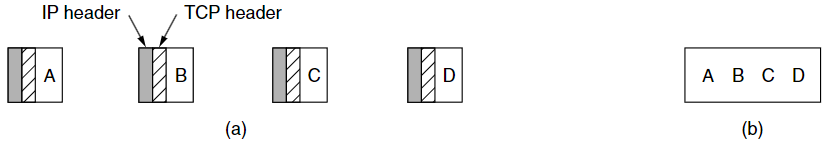
\includegraphics[width=0.42\textwidth]{pic/CN6/TCP connection is a byte stream}
    \caption{ (a) Four 512-byte segments sent as separate IP datagrams. (b) The 2048 bytes of data delivered to the application in a single READ call.}
\end{figure}

When an application passes data to TCP, TCP may send it immediately or buffer it.
\begin{itemize}
    \item PUSH flag: send immediately
    \item URGENT flag: high priority
\end{itemize}

\begin{figure}[!htb]
    \centering
    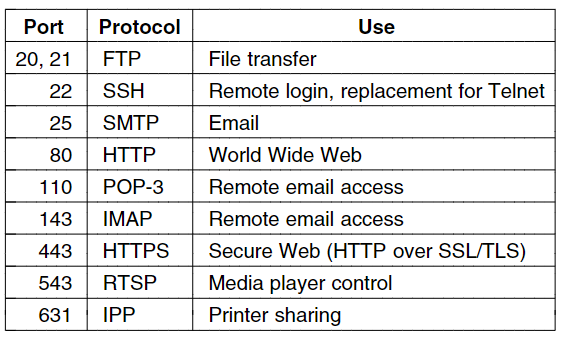
\includegraphics[width=0.309\textwidth]{pic/CN6/Some assigned ports}
    \caption{Some assigned ports}
\end{figure}

The TCP Protocol includes: a fixed 20-byte header + <optional> + <0-N data bytes>. 

The form of data exchange: segment. 

The basic TCP protocol: the sliding window protocol with dynamic window size. 

There are many problems to solve:
\begin{enumerate}
    \item Segment can arrive out of order
    \item Segments can also be delayed
\end{enumerate}

\subsubsection{The TCP Segment Header}
A key feature of TCP, and one that dominants the protocol design, is that every byte on a TCP connection has its own 32-bit sequence number. Every segment begins with a fixed-format, 20-byte header. 

Segments without any data are legal and are commonly used for acknowledgements and control messages.

\begin{figure}[!htb]
    \centering
    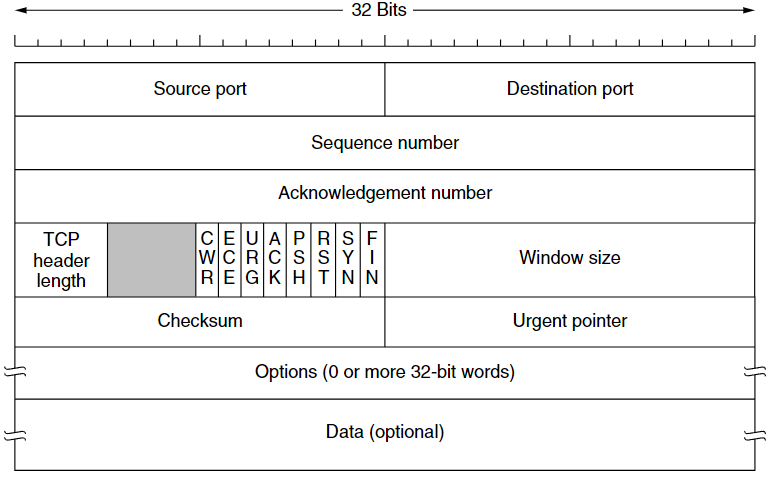
\includegraphics[width=0.42\textwidth]{pic/CN6/The TCP header}
    \caption{The TCP header}
\end{figure}

\begin{enumerate}
    \item The Source port (16 bits) and Destination port (16 bits)
    \subitem The connection identifier is a 5 tuple because it consists of five pieces of information: the protocol (TCP), source IP, and source port, and destination IP and destination port.
    \item The Sequence number (32 bits) and Acknowledgement number (32 bits) fields
    \subitem The Acknowledgement number specifies the next in-order byte expected, not the last byte correctly received.
    \subitem It is a cumulative acknowledgement because it summarizes the
    received data with a single number.
    \item The TCP header length (4 bits): because of the Options field. 
    \item The not used 4-bit field
    \item eight 1-bit fields (ack, syn, fin is important)
    \begin{itemize}\small
        \item CWR and ECE are used to signal congestion when ECN (Explicit Congestion Notification) is used.
        \subitem ECE is set to signal an ECN-Echo to a TCP sender
        \subitem CWR is set to signal Congestion Window Reduced from the TCP sender
        \item URG is set to 1 if the Urgent pointer is in use.
        \subitem The Urgent pointer is used to indicate which urgent data are to be found
        \item The ACK bit is set to 1 to indicate that the Acknowledgement number is valid
        \item The PSH bit indicates PUSHed data
        \item The RST bit is used to abruptly reset a connection
        \item The SYN bit is used to establish connections
        \begin{itemize}\scriptsize
            \item The connection request has SYN = 1 and ACK= 0
            \item SYN = 1 and ACK = 1: the connection reply does bear an acknowledgement.
        \end{itemize}
        \item The FIN bit is used to release a connection. 
        \subitem Both SYN and FIN segments have sequence numbers and are thus guaranteed to be processed in the corrected order.
    \end{itemize}
    \item The Window size field (16 bits) tells how many bytes
    may be sent starting at the byte acknowledged
    \subitem A window size field of 0 is legal, would like no more data for the moment. 
    \item Checksum (16 bits).  It checksum the header, the data and a conceptual pseudoheader. 
    \begin{figure}[!htb]
        \centering
        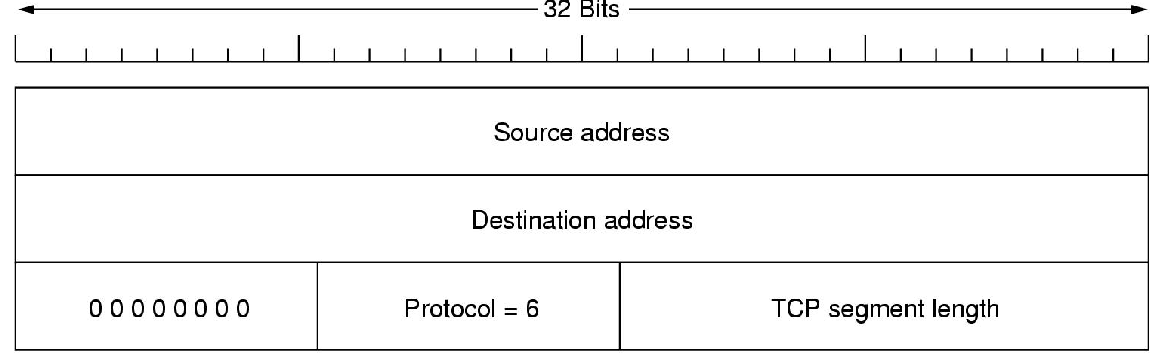
\includegraphics[width=0.42\textwidth]{pic/CN6/The pseudoheader of TCP}
        \caption{The pseudoheader of TCP}
    \end{figure}
    \item The Options field. may extended to 40 bytes to accommodate the longest TCP header 
    \begin{itemize}
        \item MSS(Maximum Segment Size), it defaults to a 536-byte load.
        \item The window scale negotiate a window scale factor at the start of a connection
        \item The timestamp 
        \item The SACK (Selective ACKnowledgement), is  used after a packet has been lost but subsequent (or duplicate) data has arrived. 
    \end{itemize}
\end{enumerate}

\subsubsection{TCP Connection Establishment}
Three Way Handshake
\begin{figure}[!htb]
    \centering
    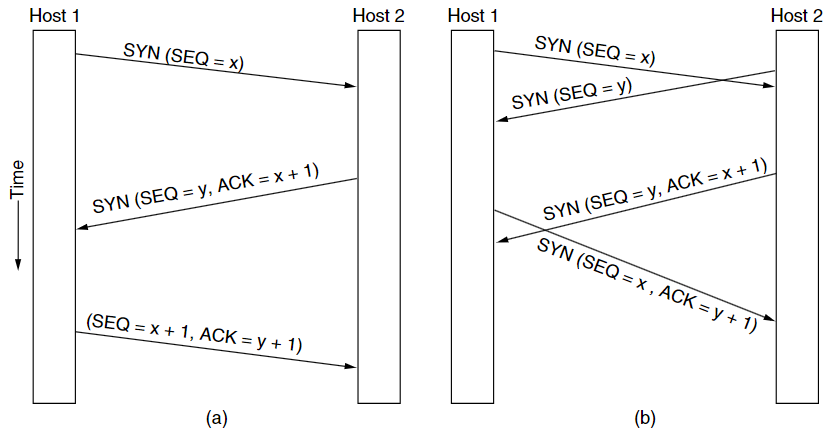
\includegraphics[width=0.42\textwidth]{pic/CN6/TCP Connection Establishment}
    \caption{(a) TCP connection establishment in the normal case. (b) Simultaneous connection establishment on both sides.}
\end{figure}

\begin{enumerate}
    \item Note that a SYN segment
    consumes 1 byte of sequence
    space so that it can be
    acknowledged unambiguously.
    \item The initial sequence number
    chosen by each host should
    cycle slowly. This rule is to
    protect against delayed
    duplicated packets.    
\end{enumerate}

\begin{enumerate}
    \item SYN --- for establishing a connection
    \subitem Request segment contains the following information in TCP header:
    \begin{enumerate}\scriptsize
        \item Initial sequence number (randomly chosen by the client)
        \item SYN bit set to 1.
        \item Maximum segment size
        \item Receiving window size (the limit of unacknowledged data that can be sent to the client, contained in the window size field)       
    \end{enumerate}
    \item SYN + ACK --- After receiving the request segment
    \subitem Reply segment contains the following information in TCP header:
    \begin{enumerate}\scriptsize
        \item Initial sequence number (randomly chosen by the server)
        \item SYN bit set to 1.
        \item Maximum segment size
        \item Receiving window size
        \item Acknowledgement number
        \item ACK bit set to 1. 
    \end{enumerate}
    \item ACK --- After receiving the reply segment
    \subitem sending a pure acknowledgement. Not necessary. 
\end{enumerate}

\paragraph{Important Points}\quad

\begin{itemize}\small
    \item Connection establishment phase consume 1 sequence number of both sides. But pure acknowledgement do not consume any sequence number. 
    \item Pure acknowledgement for the reply segment is not necessary. Client sending the data packet immediately can be considered as an ack. 
    \item For all the segments except the request segment, ACK bit is always set to 1.
    \item Certain parameters are negotiated during connection establishment. 
    \begin{enumerate}
        \item Window size
        \item Maximum segment size
        \item Timer values
    \end{enumerate}
    \item In any TCP segment
    \begin{itemize}\scriptsize
        \item If SYN bit = 1 and ACK bit = 0, then it must be the request
        segment.
        \item If SYN bit = 1 and ACK bit = 1, then it must be the reply segment.
        \item If SYN bit = 0 and ACK bit = 1, then it can be the pure ACK or segment meant for data transfer.
        \item If SYN bit = 0 and ACK bit = 0, then this combination is not possible.
    \end{itemize}
\end{itemize}

\paragraph{\textbf{SYN Flood} Attack} A malicious sender 发送大量 SYN segments, 但不完成链接.

用 SYN cookies 对抗. 即将 sequence number hash, 这样接受时只需要比对 hash 是否一致. 

\subsubsection{TCP Connection Release}
\begin{figure}[!htb]
    \centering
    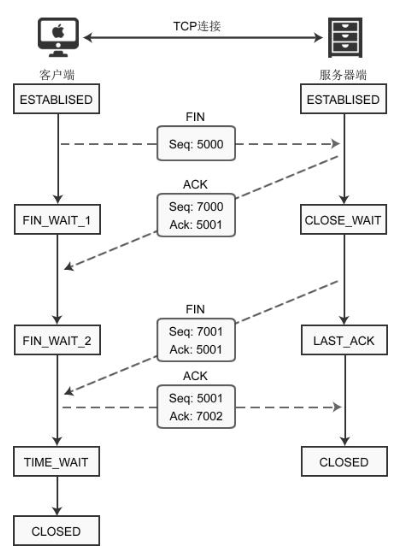
\includegraphics[width=0.22\textwidth]{pic/CN6/TCP Connection Release}
    \caption{TCP Connection Release}
\end{figure}

Four TCP segments are needed to release a connection: one FIN and one ACK for each direction. 

\textbf{The Two-army Problem}: 需要知道信号是否送达. 

The following steps are followed in terminating the connection:
\begin{enumerate}\scriptsize %TODO 62-63
    \item For terminating the connection
    \item after receiving the FIN segment
    \item After receiving the acknowledgement, client enters the state called FIN\_WAIT\_2. Now
    \item Now suppose server wants to close the connection with the client. For terminating the connection
    \item After receiving the FIN segment
\end{enumerate}

\begin{figure}[!htb]
    \centering
    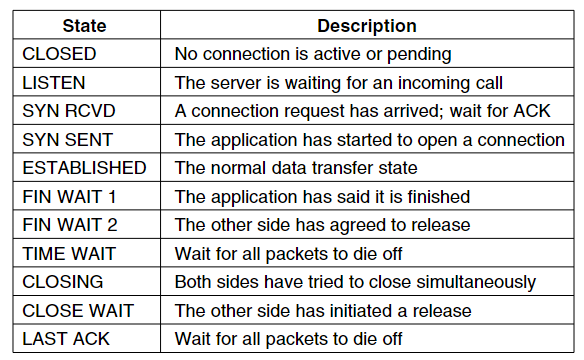
\includegraphics[width=0.309\textwidth]{pic/CN6/The states used in the TCP connection management finite state machine}
    \caption{The states used in the TCP connection management finite state machine}
\end{figure}

\begin{figure}[!htb]
    \centering
    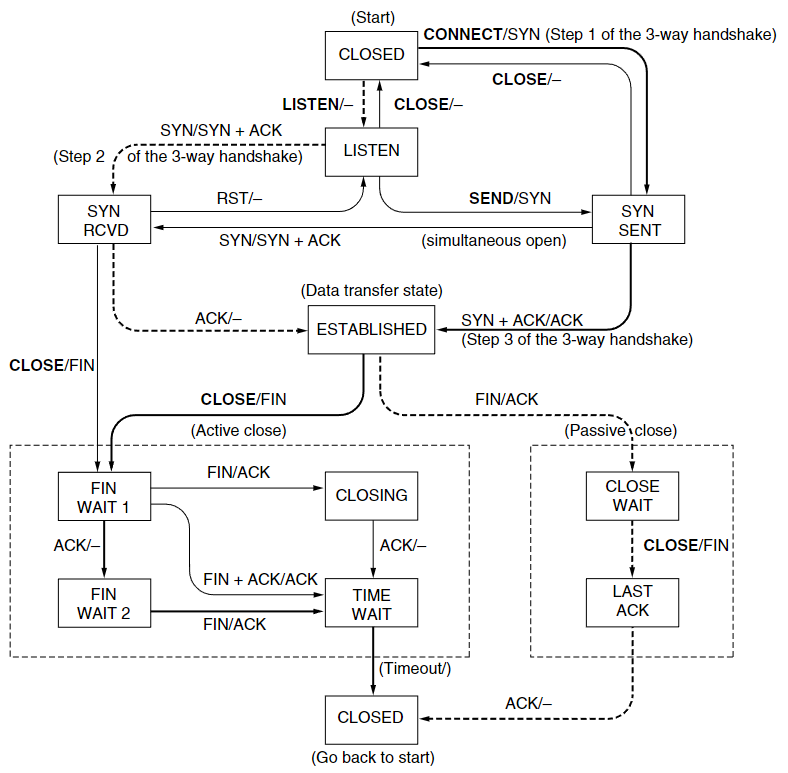
\includegraphics[width=0.42\textwidth]{pic/CN6/TCP connection management finite state machine}
    \caption{TCP connection management finite state machine}
\end{figure}


\subsubsection{TCP Sliding Window}

\begin{figure}[!htb]
    \centering
    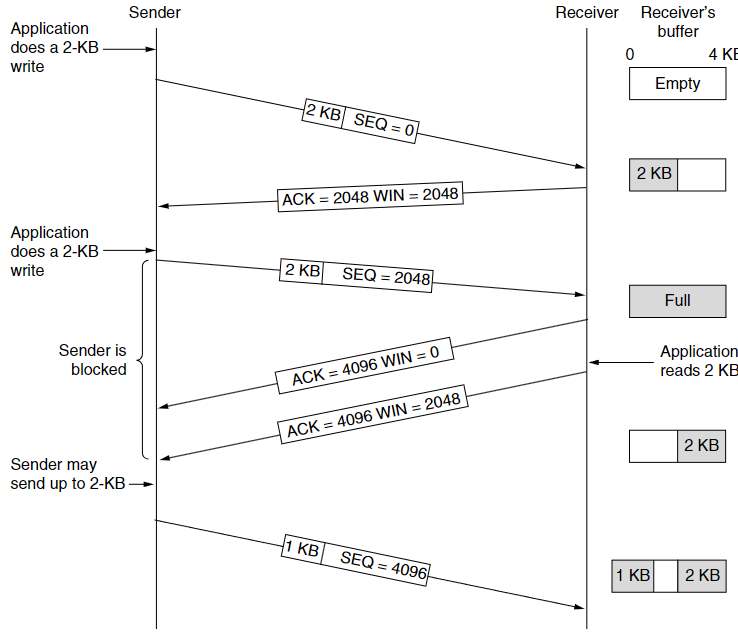
\includegraphics[width=0.22\textwidth]{pic/CN6/Window management in TCP}
    \caption{Window management in TCP}
\end{figure}

Example %TODO 70-72
syn + ack 需要占用一个 sequence number, 纯 ack 不用占用. 每个 byte 都有一个对应的 sequence number, 这个 sequence number 也可以携带 ack. 

\begin{figure}[!htb]
    \centering
    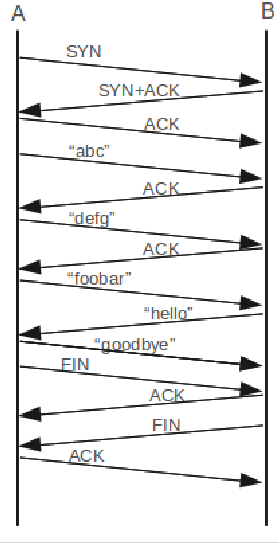
\includegraphics[width=0.1\textwidth]{pic/CN6/An Ladder Example}
    \caption{An Ladder Example}
\end{figure}

\begin{figure}[!htb]
    \centering
    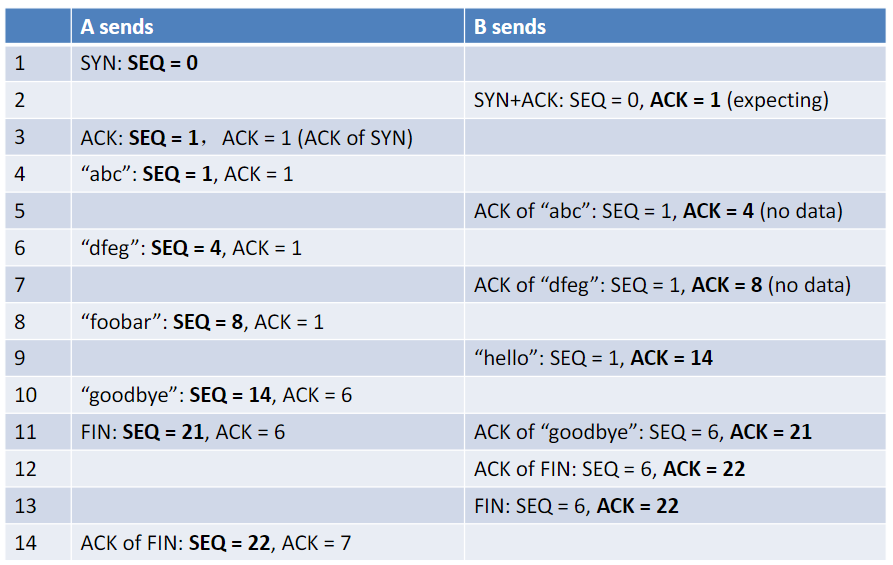
\includegraphics[width=0.309\textwidth]{pic/CN6/An Ladder Example2}
    \caption{An Ladder Example}
\end{figure}

%TODO p72
% 2 ack=20001
% 3 seq=20001 ack=5001
% 4 seq=20001 ack=5001
% 5 seq=5001 ack=21001
% 6 seq=21001 ack=5001
% 7 seq=5001 ack=22001
% 8 seq=22001 ack=5001
% 9 seq=5001 ack=23001
% 10 seq=5001 ack=23001
% 11 seq=23001 ack=6001
% 12 seq=6001 ack=23001


When the window is 0, the sender may not normally send segments, with two exceptions:
\begin{enumerate}\scriptsize
    \item Urgent data may be sent, for example, to allow the user to
    kill the process running on the remote machine
    \item The sender may send a 1-byte segment to force the receiver
    to re-announce the next byte expected and the window size.
    This packet is called a window probe
\end{enumerate}

\paragraph{Nagle's Algorithm}To reduce the bandwidth used by a sender that sends multiple short packets. 当有数据要发送, 先发送一个分片, 缓存其他分片, 受到ack 后一次性发送缓存的分片. 但因为缓存, 高交互系统可能造成死锁. 

\paragraph{Clark's Solution} the silly window syndrome: an interactive application on the receiving side reads data only 1 byte at a time. 只有 receiver 有一定比例的 window 可用后再通知 sender. 

\paragraph{The Silly Window Syndrome}The goal is for the sender not to send small segments and the receiver not to ask for them. 


Another issue that the receiver must handle is that segments may arrive out of order. Solution:
\begin{itemize}\scriptsize
    \item The receiver will buffer the data until it can be passed up to the
    application in order
    \item Acknowledgements can be sent only when all the data up to byte
    acknowledged have been received. This is called a cumulative acknowledgement
\end{itemize}

\subsubsection{TCP timer management}
TCP uses multiple timers (at least conceptually) to do its
work.
\begin{itemize}
    \item The RTO (Retransmission TimeOut)
    \subitem How long should the RTO be ? 
    \item The Persistence timer
    \item The Keepalive timer
    \item The one used in TIME WAIT state
\end{itemize}

\paragraph{The RTO (Retransmission TimeOut)}\quad 

\begin{itemize}
    \item set too short, unnecessary retransmissions will occur.
    \item set too long, performance will suffer due to the long retransmission delay whenever a packet is lost
\end{itemize}
Furthermore, the ack arrival can change rapidly within a few seconds as
congestion builds up or is resolved

The solution is to use a dynamic algorithm: 
\begin{itemize}\scriptsize
    \item SRTT (Smoothed Round-Trip Time, Jacobson,1988)
    \subitem Exponentially Weighted Moving Average (EWMA, R is the current
    estimate of the RTT)
    \begin{align*}
        SRTT=\alpha SRTT+(1-\alpha)R 
    \end{align*}
    where $\alpha =7/8$. 
    \item RTTVAR (Round-Trip Time VARiration)
    \subitem To make the timeout value sensitive to the variance in round-trip times as well as the smoothed round-trip time.
    \begin{align*}
        RTTVAR &=\beta RTTVAR +(1-\beta) |SRTT-R|\\
        RTO&=SRTT +4\times RTTVAR\\
        RTO&=\min(1 sec , RTO)
    \end{align*}
    where $\beta=3/4$
\end{itemize}


One problem that occurs with gathering the samples, R, of the round-trip time is what to do when a segment times out and is sent again. 但当接受 ack 时无法确定是从发的 ack 还是先前的 ack. 

Karn's algorithm: 重传的 rtt 不参与更新 rto. 每次失败的重传 timeout doubled. 

\paragraph{the persistent timer}It is designed to prevent the following deadlock %TODO 85

\paragraph{the keepalive timer}看看对方是否下线. 

\paragraph{the TIME WAIT timer}twice the maximum packet lifetime

\subsubsection{TCP Congestion Control}
The network layer 满了只能 dropping packets(丢包). 所以靠 transport layer 解决. In the Internet, TCP plays the main role in controlling congestion, as well as the main role in reliable transport. 

TCP congestion control is based on a AIMD (Additive
Increase Multiplicative Decrease) control law using a
window and with packet loss(丢包) as the binary signal.

TCP maintains a congestion window(the sending window) and a flow control window(the receiving window):
\begin{itemize}
    \item The congestion window size 是指每时 sender 最大发送的字节数. 
    \subitem The corresponding rate = window size/RTT
    \subitem TCP 用 AIMD 调整 congestion window size
    \item The flow control window size 是指每时最大容纳的字节数. Receiver 通过 TCP Header 告知 sender 其 window size. 
    \subitem 发送字节数应该同时小于 两 window size
    \subitem 任意 window size full, TCP 停止传输数据. 
\end{itemize}

All the Internet TCP algorithms assume that lost packets(丢包) are caused by congestion and monitor timeouts. 

During the implementation, we have two important questions:
\begin{enumerate}\scriptsize
    \item The transmission rate of packets which the sender will use
    \subitem ack clock
    \item The size of the congestion window
    \subitem slow start
\end{enumerate}

%TODO 96
The key observation is that ack 到 sender 的 rate 受 slowest link 制约.
The acknowledgements reflect the times at which the packets arrived at
the receiver after crossing the slow link.
This timing is known as an ack clock. It is an essential part of TCP

\begin{figure}[!htb]
    \centering
    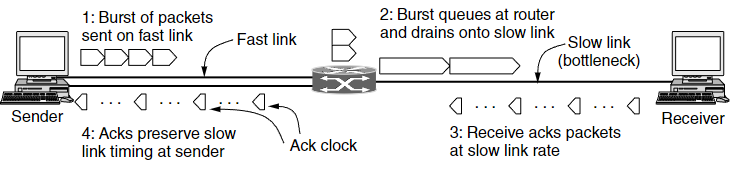
\includegraphics[width=0.42\textwidth]{pic/CN6/A burst of packets from a sender and the returning ack clock}
    \caption{A burst of packets from a sender and the returning ack clock}
\end{figure}

\paragraph{TCP Start Problem}We want to quickly near the right rate, $cwnd_{IDEAL}$. 

Slow-Start Solution: Start by doubling cwnd (the congestion window) every RTT. 每收到一个ACK, 就增加一个数据包, 也就是一个变两个. 
\begin{figure}[!htb]
    \centering
    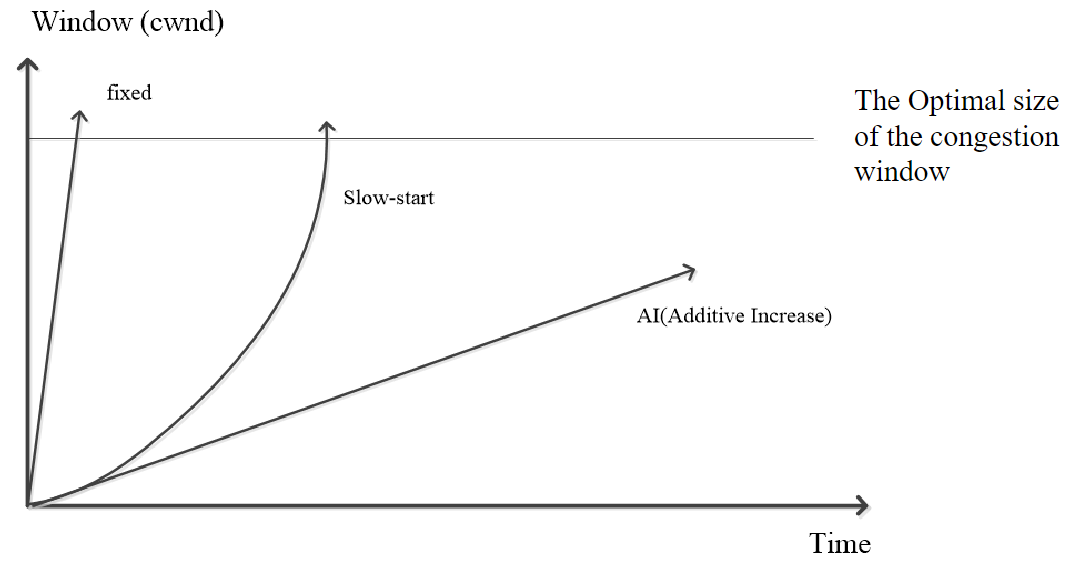
\includegraphics[width=0.309\textwidth]{pic/CN6/Slow-Start Solution}
    \caption{Slow-Start Solution}
\end{figure}

To keep slow start under control, the sender keeps a threshold for the connection called the slow start threshold (sst).
\begin{itemize}
    \item 起始设置为 flow control window size. 
    \item TCP keeps increasing the congestion window in slow start until
    \begin{enumerate}
        \item a timeout occurs (packet loss): sst 降到 congestion window 的一半, 且重启 slow start. 
        \item the congestion window exceeds the slow start threshold: 从 slow start 变为 additive increase (线性)
    \end{enumerate}
\end{itemize}

additive increase: 完成一个完整的RTT, 才增加一个数据包. 

\begin{figure}[!htb]
    \centering
    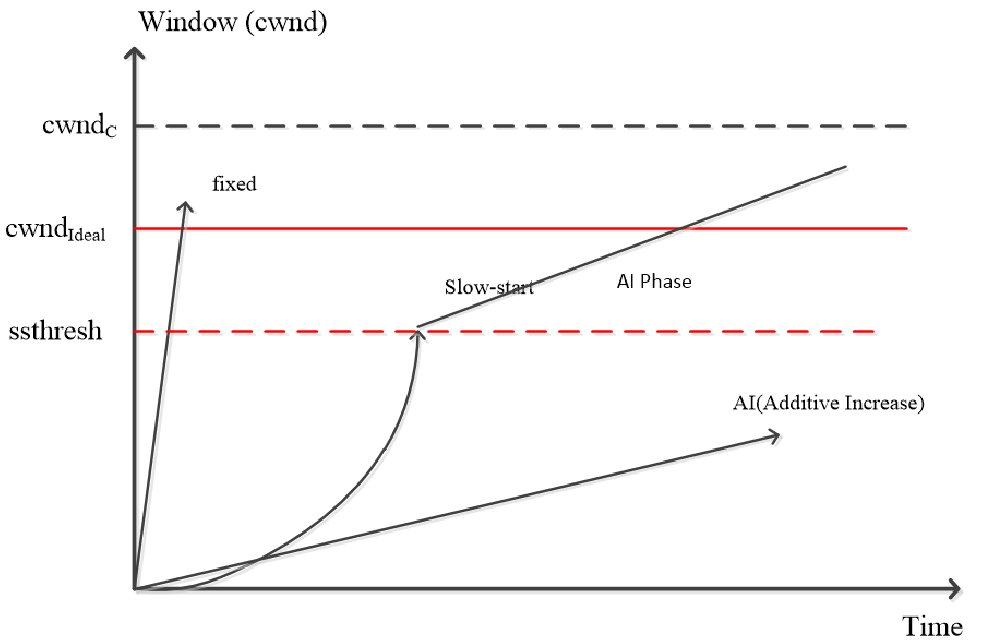
\includegraphics[width=0.309\textwidth]{pic/CN6/A mix of linear and the multiplication increase}
    \caption{A mix of linear and the multiplication increase}
\end{figure}

\paragraph{Inferring Loss from ACKs}\quad 
\begin{itemize}
    \item TCP uses a cumulative ACK
    \item Duplicate ACKnowledgements gives us hints about what data hasn't arrived
    \begin{itemize}
        \item 告知收到数据包, 但不是期望的
        \item 将三次相同的 ack 当作 loss
        \item 即使计时器没有 timeout, 但也做重传 (Fast Retransmission)
        \item sst 设置为 congestion window/2, slow start 重启
    \end{itemize}
\end{itemize}

\paragraph{Fast Retransmission}It can repair single segment loss quickly, typically before a timeout %TODO 104 + 12.5 钉钉


\paragraph{Fast Recovery}Fast recovery is the heuristic that implements this behavior
\begin{itemize}%TODO 109
    \item pretend further duplicate ACKs are the expected ACKs
    \item duplicate ACKs are counted (including the three that
    triggered fast retransmission) until the number of packets in the
    network has fallen to the new threshold
    \item Reconcile views when the ACK jumps
\end{itemize}


Two larger changes have also affect TCP implementations
\begin{enumerate}
    \item SACK (Selective ACKnowledgements) 
    \begin{figure}[!htb]
        \centering
        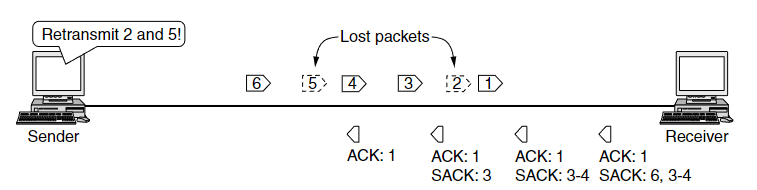
\includegraphics[width=0.42\textwidth]{pic/CN6/Selective acknowledgements}
        \caption{Selective acknowledgements}
    \end{figure}
    \item ECN (Explicit Congestion Notification): an IP layer mechanism
    \begin{itemize}
        \item ECE (ECN-Echo): tell the TCP sender to slow down
        \item CWR: The sender tells the receiver that it has heard the signal
    \end{itemize}
\end{enumerate}

TCP Reno, NewReno, and SACK. (笔记中没有前两个版本)
\begin{itemize}\scriptsize
    \item Reno can repair one loss per RTT
    \subitem Multiple losses cause a timeout
    \item NewReno further refines ACK heuristics
    \subitem Repairs multiple losses without timeout
    \subitem SACK (Selective Acknowledgement) is a better idea
\end{itemize}

\subsection{Introduce new transport layer protocols}
\subsubsection{QUIC} 
全称 (Quick UDP Internet Connection), 中文翻译成 ``快速 UDP 互联网连接'', 是由 Google 提出的使用 UDP 进行多路并发传输的协议. 

%TODO 自己去看 120- 

\begin{enumerate}
    \item Low latency to establish connection
    \item Improved Congestion Control Scheme
    \item reliable transmission based on monotonically increased packed number. 
    \subitem Stream offset
    \item removal of the ``Head-of-Line blocking'' (HOL blocking) problem (队头阻塞问题)
    \item 连接迁移
\end{enumerate}

\subsubsection{BBR} 
(Congestion Control based on Bottleneck Bandwidth)

%TODO 自己去看 130-

现在丢包与拥塞不再等价了. 

A full-duplex TCP connection has exactly one slowest link or bottleneck in each direction. The bottleneck is important because It determines the connection's maximum data-delivery rate. 

Two physical constraints, RTprop (round-trip propagation time) and BtlBw (Bottleneck Bandwidth), bounds transport performance. If the network path were a physical pipe, Rtprop would be its length and BtlBW its minimum diameter. 

\begin{figure}[!htb]
    \centering
    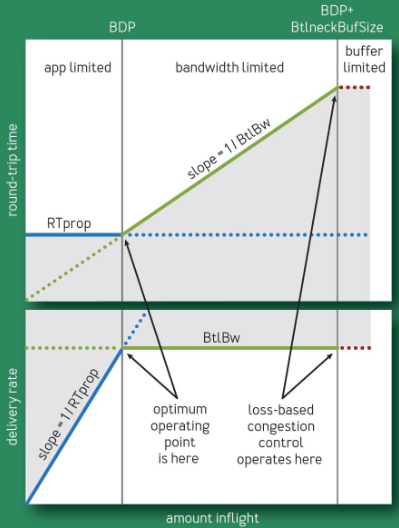
\includegraphics[width=0.309\textwidth]{pic/CN6/bbr.png}
    \caption{RTT and delivery rate variration with the amount of data inflight}
\end{figure}

data in flight (data sent but not yet acknowledged) = BtlBw $\times$ Rtprop

Bandwidth-delay product (BDP) is a measurement of how many bits can fill up a network link

Little's Result:
\begin{align*}
    \bar{N}=\lambda T
\end{align*}
\begin{itemize}
    \item $\bar{N}$ is the data in flight in the network
    \item $T$ RTT
    \item $\lambda$ the delivery rate
\end{itemize}

\begin{align*}
    T&=\frac{\bar{N}}{\lambda}=\frac{\bar{N}}{BtlBw}=RTT\\
    \lambda&=\frac{\bar{N}}{T}=\frac{\bar{N}}{RTprop}
\end{align*}

Rtprop and BtlBw obey an uncertainty principle: whenever one can measured, the other cannot.

Characterizing the bottleneck:
\begin{itemize}
    \item Rate balance
    \item Full pipe
    \item BtlBw and RTprop vary over the life of a connection, so they must be continuously estimated
\end{itemize}